\documentclass{article}

\usepackage[utf8]{inputenc}
\usepackage[T1]{fontenc}
\usepackage[polish]{babel}
\usepackage{longtable}
\usepackage{amsmath}

\usepackage{chemformula}
\title{lab7}
\author{adamch08 }
\date{November 2018}

\usepackage{natbib}
\usepackage{graphicx}

\begin{document}
% strona tytułowa
\titlepage
Strona tytułowa
% spis treśći
\tableofcontents

\maketitle
\section{Sekcja}
Tekt sekcji
\subsection{Subsekcja}
Tekst subsekcji
\subsubsection{Subsubsekcja}
Tekst subsubsekcji
\paragraph{paragraf 1} ~\\
%\textbf - pogrubienie
%\emph - wyróżnienie
%\texttt - pismo o jednakowej szerokości znaków, teletypefont family
%\textit - kursywa
%\textsc - kapitaliki
%\textnormal - główny font dokumentu
The fact that half of all \textbf{Americans} with \textit{health insurance} get it through their jobs is a true oddity of the U.S. health care \texttt{system}.
\paragraph{paragraf 2} ~\\
No other country operates in such a way. Yet surveys show that most people on employer-sponsored health insurance (\emph{ESHI}) seem to be \textnormal{happy} with it.
\paragraph{paragraf 3} ~\\
So why shouldn’t we follow the old maxim “If it ain’t broke, don’t \textsc{fix} it?”.

\subparagraph{Subparagraf} ~\\
Tekst subparagrafu
%intrukcja zmieniająca numberację z cyfr na litery (dotyczy punktów w klasie article)
\appendix

\section{Zadanie 4 - Listy}
% lista numerowana
\paragraph{Trudne egaminy w sesji zimowej}
\begin{enumerate}
    \item[--]
    \begin{enumerate}
        \item Podstawy ochrony danych
        \item Systemy wbudowane
        \item Platformy programowania
    \end{enumerate}
\end{enumerate}

% lista punktowana
\paragraph{Poznane języki programowania}
\begin{itemize}
    \item Java
    \item C~++
    \item C\#
    \item PHP
\end{itemize}
\section{Zadanie 5 - Cudzysłowy}
% cudzysłów angielski
``Marcin to kocur''~\\
% cudzysłów francuski
<<Marcin to kocur>>~\\
% cudzysłów polski
,,Marcin to kocur\footnote{Głupek}''~\\

\section{Zadanie 6 - Wstawki}
%obraz
% znaki określające dopuszczalny sposób umiszczenia wstawki
% h, t ,b, p, !
% h - bez przemiszczenia, dokładnie w miejscu użycia
% t - na górze strony 
% b - na dole strony
% p - na stronie zawierającej wyłącznie wstawki
% ! - ignorując większość parametrów kontrojuących umiszczanie wstawek (np. max dopuszczalna liczba wstawek na stronie)

\begin{figure}[h!]
\centering
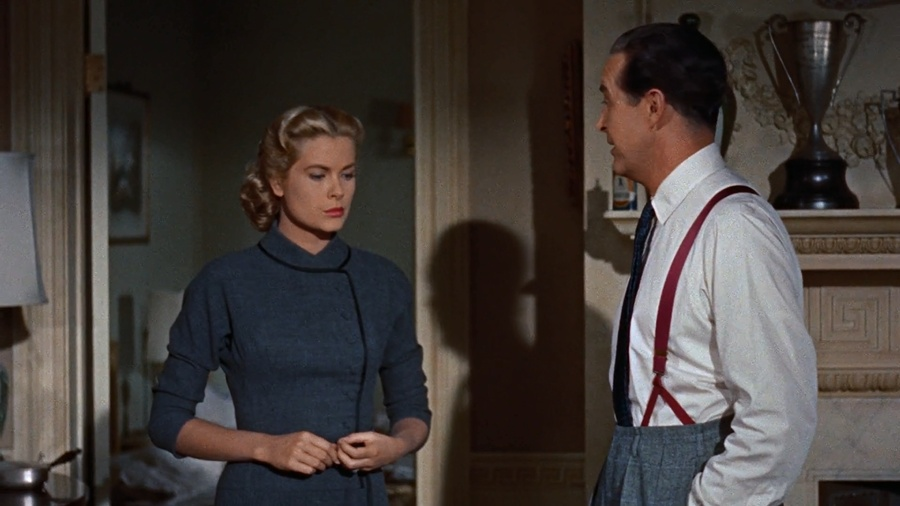
\includegraphics[scale=0.3]{DialMforMurder}
\caption{Dial M for Murder}
\label{fig:murder}
\end{figure}
% l - dosunięcie zawartości do lewej 
% c - do środka
% r - do prawej
% \hline - pozioma kreska
% 
\begin{center}
    \begin{longtable}{|l | c | r|}
     \caption{Zestawienie województw} 
      \label{tab:woj} \\ \hline
        Województwo & Powierzchnia w km$^{2}$ & Populacja \\ \hline
        \endhead
        Dolnośląskie & 19 947 & 2 902 365 \\ \hline
        Kujawsko-pomorskie & 17 972 & 2 082 935 \\ \hline
        Lubelskie & 25 122 & 2 129 260 \\
        \hline
       
    \end{longtable}
\end{center}

Rysunek~\ref{fig:murder} przedstawia kadr z filmu~\pageref{fig:murder}.~\\
Tabela~\ref{tab:woj}  na stronie ~\pageref{tab:woj} przedstawia zestawienie województw.

\section{Zadanie 7 - równania matematyczne}
{\Huge
$\binom{n}{k} = \frac{n!}{k!(n-k)!}$~\\\\\\
$a^2 + b^2 = c^2$~\\\\\\
$\frac{\frac{1}{2}+\frac{1}{4}}{\frac{1}{8}} \neq 1$~\\\\\\

\begin{displaymath}
\sum_{i=1}^{n} i^2 
= \frac{n(n+1)(2n+1)}{6}
\end{displaymath}
~\\\\\\
\ch{C2^{-3} + O2^0 -> C^{+4}O2^{-2} + H2^{+1}O^{-2}}
~\\\\\\
$A_{m,n} = 
 \begin{pmatrix}
  a_{1,1} & a_{1,2} & \cdots & a_{1,n} \\
  a_{2,1} & a_{2,2} & \cdots & a_{2,n} \\
  \vdots  & \vdots  & \ddots & \vdots  \\
  a_{m,1} & a_{m,2} & \cdots & a_{m,n} 
 \end{pmatrix}$
}

\section{Conclusion}
``I always thought something was fundamentally wrong with the universe'' \citep{adams1995hitchhiker}~\\
<<Ludzie sypiają ze sobą, nic ekscytującego. Zdjąć przed kimś ubrania i położyć się na kimś, pod kimś>> \citep{jakub2018zulczyk}~\\
,,Ktokolwiek ratuje jedno życie, jakby cały świat ratował."" \citep{heather2018morris}~\\
``I przedmioty już wiedziały. Czuły, że wkrótce będą przesuwane. Przekładane w niewłaściwie miejsca.''
\citep{marcin2017wicha}~\\

\bibliographystyle{plain}
\bibliography{references}
\end{document}
